\chapter{Implementación y Migración}
\label{chap:Implementacion}
\textit{This chapter introduces the theoretical, experimental and computational concepts used throughout the thesis}
\vspace{2ex}\vfill
\minitoc
\newpage

\section{Punto de Vista de Proyecto}
Un punto de vista del proyecto se utiliza principalmente para modelar el cambio de arquitectura. El proceso de migración de la “arquitectura” desde una situación o estado anterior a una nueva situación tiene consecuencias importantes en la estrategia de crecimiento a largo y mediano plazo, y el proceso de toma de decisiones. Algunas de las cuestiones que deben tenerse en cuenta por los modelos diseñados en este punto de vista son:
  
  \begin{itemize}
  	\itemcolor{azull}
	\item El desarrollo de la arquitectura empresarial en toda la organización es una tarea que puede requerir varios años.
	\item Todos los sistemas y servicios deben seguir funcionando sin importar todas las modificaciones presumibles y cambios en la arquitectura de la empresa durante el proceso de cambio.
	\item El proceso de cambio puede tener que lidiar con estándares tecnológicos inmaduros (por ejemplo, mensajería, seguridad, datos, etc.).
	\item El cambio tiene consecuencias graves para el personal, la cultura, la forma de trabajo y la organización.
  \end{itemize}

  \begin{table}[H]
	\centering
	\begin{tabular}{p{3.7cm}p{8cm}}
		\hline
		\rowcolor{azull}
		{\color{blancoo} \textbf{Nombre}} & {\color{blancoo} \textbf{Proyecto}} \\
		\hline
		\textbf{Stakeholders} & Gerentes (operativos), empresarios, arquitectos TIC, empleados, accionistas \\
		\textbf{Preocupaciones} & Visión y políticas de la arquitectura, motivación \\
		\textbf{Propósito} & Decidir, informar \\
		\textbf{Nivel de Abstracción} & Conjunto \\
		\textbf{Capa} & Capa de implementación y migración \\
		\textbf{Aspectos} & Estructura pasiva, comportamiento, estructura activa \\
		\bottomrule
	\end{tabular}
	\captionsetup{width=.95\textwidth}
	\caption{Descripción punto de vista del proyecto}
	\label{tabla26}
  \end{table}

  \begin{figure}[H]
	\centering
	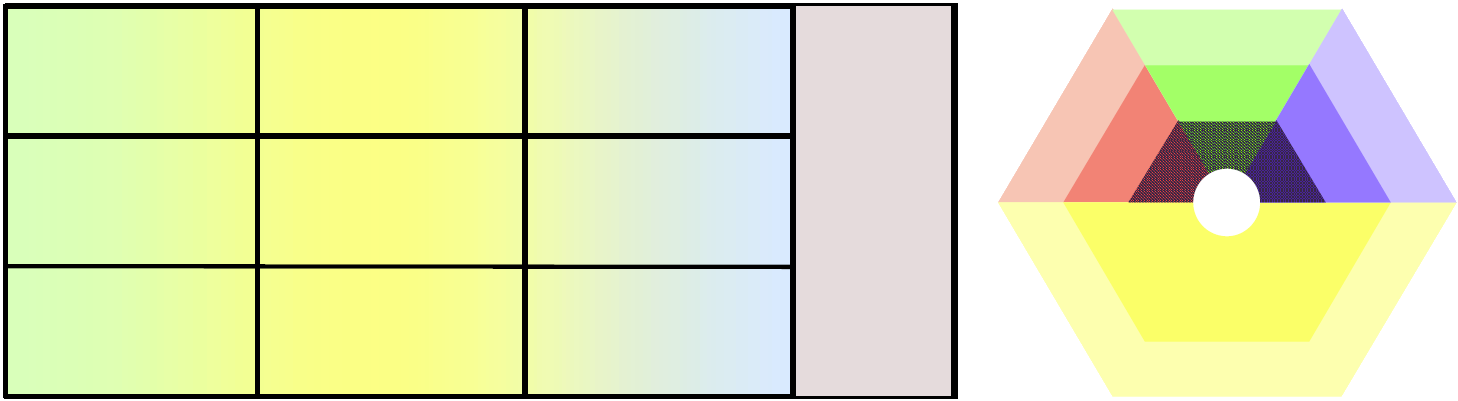
\includegraphics[scale=0.2]{figuras/35}
	\captionsetup{width=.95\textwidth}
	\caption{Posición del punto de vista del proyecto conceptualmente y marco del punto de vista}
	\label{figura35}
  \end{figure}

  \subsection{Metamodelo}
  En la Figura 10.1 se ilustra el metamodelo del punto de vista de Proyecto donde se resuelven los objetivos a partir de paquetes de trabajo, el paquete de trabajo es el conjunto de actividades con miras a generar entregables, esto está asociado a roles que a su vez está asignado a actores; los paquetes resuelven objetivos.

  \begin{figure}[H]
	\centering
	\includegraphics{metamodelos/23}
	\captionsetup{width=.95\textwidth}
	\caption{Metamodelo punto de vista del proyecto}
	\label{metamodelo23}
  \end{figure}

  \subsection{Modelo mInstituto}
  En la vista se representa el vínculo existente entre elementos de la vista de motivación y los componentes presentes en la vista de negocio donde el objetivo de negocio principal es el de proveer soluciones tecnológicas que permitan optimizar la gestión de la información en las instituciones educativas, a este objetivo se encuentran asociados los roles principales de negocio, es decir, el desarrollador y el cliente.  El paquete de trabajo unido al objetivo corresponde al desarrollo de la solución tecnológica.
  
  \begin{figure}[H]
	\centering
	\includegraphics[scale=0.65]{modelos/23}
	\captionsetup{width=.95\textwidth}
	\caption{Modelo punto de vista del proyecto: minstituto}
	\label{modelo23}
  \end{figure}
  
\section{Punto de Vista de Migración}
El punto de vista de migración implica modelos y conceptos que pueden ser utilizados para especificar la transición de una arquitectura existente a una arquitectura deseada. \\
El punto de vista de migración implica modelos y conceptos que pueden ser utilizados para especificar la transición de una arquitectura existente a una arquitectura deseada.

  \begin{table}[H]
	\centering
	\begin{tabular}{p{3.7cm}p{8cm}}
		\hline
		\rowcolor[HTML]{0073a1}
		{\color[HTML]{FFFFFF} \textbf{Nombre}} & {\color[HTML]{FFFFFF} \textbf{Migración}} \\
		\hline
		\textbf{Stakeholders} & Arquitectos empresariales, arquitectos de proyecto, arquitectos de aplicación, arquitectos de dominio, arquitectos de infraestructura, empleados \\
		\textbf{Preocupaciones} & Historia de los modelos \\
		\textbf{Propósito} & Diseñar, decidir, informar \\
		\textbf{Nivel de Abstracción} & Conjunto \\
		\textbf{Capa} & Capa de implementación y migración \\
		\textbf{Aspectos} & NA \\
		\bottomrule
	\end{tabular}
	\captionsetup{width=.95\textwidth}
	\caption{Descripción punto de vista de migración}
	\label{tabla27}
  \end{table}

  \begin{figure}[H]
	\centering
	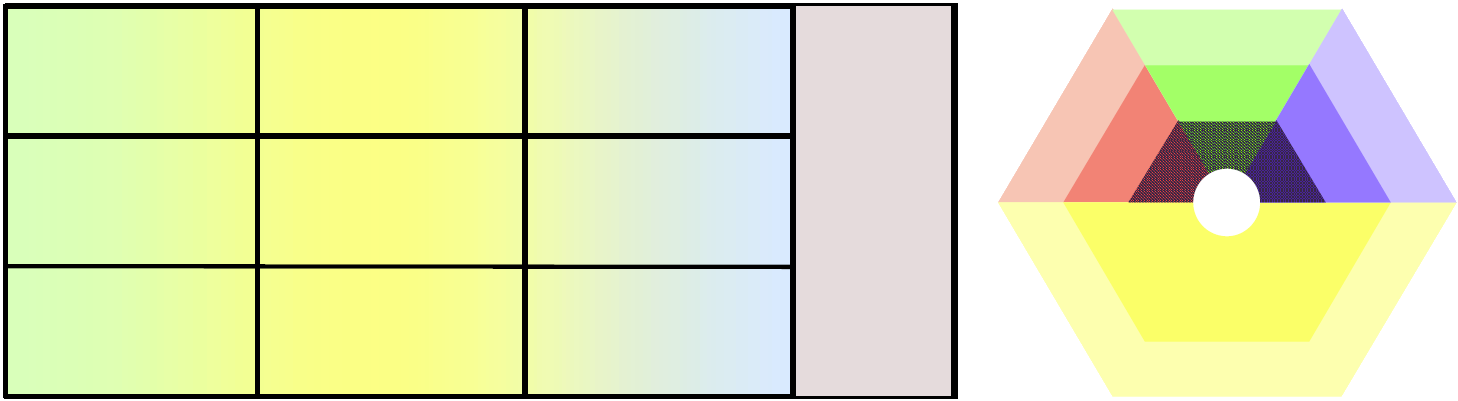
\includegraphics[scale=0.2]{figuras/35}
	\captionsetup{width=.95\textwidth}
	\caption{Posición del punto de vista de migración conceptualmente y marco del punto de vista}
	\label{figura36}
  \end{figure}

  \subsection{Metamodelo}
  En la Figura 10.3 se ilustra el metamodelo del punto de vista de Migración, En este punto de vista están los conceptos de brecha y platea, se deben tener en cuenta los hitos y como se puede pasar de un hito a otro. Una brecha es lo que se debe superar para alcanzar el otro lado, la platea es el hito en el que nos apoyamos para progresar en la arquitectura empresarial.

  \begin{figure}[H]
	\centering
	\includegraphics{metamodelos/24}
	\captionsetup{width=.95\textwidth}
	\caption{Metamodelo punto de vista de migración}
	\label{metamodelo24}
  \end{figure}

  \subsection{Modelo mInstituto}
  En la vista se representan las plateas y brechas evidenciadas para el proyecto.  Se identificaron como primera platea los requerimientos de la gestión de información de las instituciones educativas; la segunda platea es el análisis y diseño, la brecha entre las dos plateas corresponde al levantamiento de requerimientos, el cual se realiza con la información obtenida de los requerimientos.  La tercera platea corresponde al licenciamiento y la brecha entre análisis y diseño y el licenciamiento es el proceso de desarrollo del software y las pruebas correspondientes.
  
  \begin{figure}[H]
	\centering
	\includegraphics[scale=0.7]{modelos/24}
	\captionsetup{width=.95\textwidth}
	\caption{Modelo punto de vista de migración: minstituto}
	\label{modelo24}
  \end{figure}
  
\section{Punto de Vista de Migración e Implementación}
El punto de vista de la implementación y migración se utiliza para relacionar los programas y proyectos con las partes de la arquitectura que se implementan. Esta visión permite el modelado del alcance de los programas, proyectos, actividades del proyecto en términos de los elementos individuales de la arquitectura que se ven afectados. Además, se puede indicar la forma en que los elementos se ven afectados por las relaciones entre componentes.

  \begin{table}[H]
	\centering
	\begin{tabular}{p{3.7cm}p{8cm}}
		\hline
		\rowcolor[HTML]{0073a1}
		{\color[HTML]{FFFFFF} \textbf{Nombre}} & {\color[HTML]{FFFFFF} \textbf{Migración e Implementación}} \\
		\hline
		\textbf{Stakeholders} & Gerentes (operativos), organización, arquitectos TIC, empleados, accionistas \\
		\textbf{Preocupaciones} &  Visión y políticas de la arquitectura, motivación \\
		\textbf{Propósito} & Diseñar, informar \\
		\textbf{Nivel de Abstracción} & Conjunto \\
		\textbf{Capa} & Capa de negocio, Aplicación, tecnología, implementación y extensión de la migración \\
		\textbf{Aspectos} & Estructura pasiva, comportamiento, estructura activa \\
		\bottomrule
	\end{tabular}
	\captionsetup{width=.95\textwidth}
	\caption{Descripción punto de vista de la implementación y migración}
	\label{tabla28}
  \end{table}

  \begin{figure}[H]
	\centering
	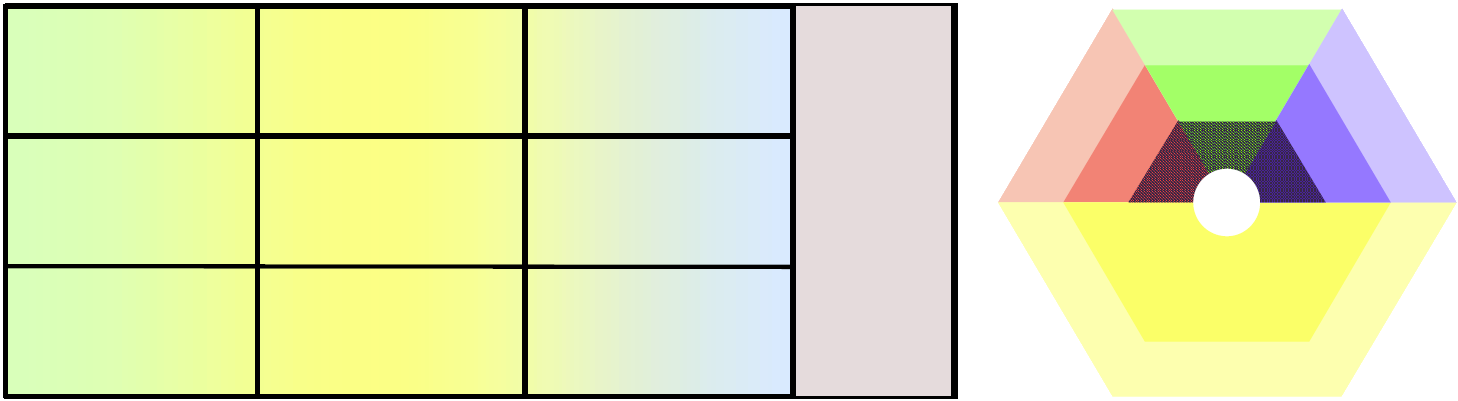
\includegraphics[scale=0.2]{figuras/35}
	\captionsetup{width=.95\textwidth}
	\caption{Posición del punto de vista de la implementación y migración conceptualmente y marco del punto de vista}
	\label{figura37}
  \end{figure}

  \subsection{Metamodelo}
  En la figura Figura 10.3 se ilustra el metamodelo del punto de vista de Migración e Implementación, es la conjunción integración de los puntos de vista de proyecto y de migración, es una síntesis del despliegue, nos resume el proyecto y la migración.

  \begin{figure}[H]
	\centering
	\includegraphics{metamodelos/25}
	\captionsetup{width=.95\textwidth}
	\caption{Metamodelo punto de vista de la implementación y migración}
	\label{metamodelo25}
  \end{figure}

  \subsection{Modelo mInstituto}
  En la vista se evidencia el paquete de trabajo que es el desarrollo de la solución tecnológica, su objetivo es proveer soluciones tecnológicas de gestión de información de las instituciones educativas, para el cumplimiento del objetivo se identificaron instrumentos puntuales que permiten su ejecución los cuales son, requerimientos específicos del negocio, análisis y diseño y el licenciamiento con sus respectivas brechas.  Se identifica como punto de unión entre los modelos de migración y proyecto el software con los requerimientos de la gestión de información de las instituciones educativas.
  
  \begin{figure}[H]
	\centering
	\includegraphics[scale=0.64]{modelos/25}
	\captionsetup{width=.95\textwidth}
	\caption{Modelo punto de vista de la implementación y migración: minstituto}
	\label{modelo25}
  \end{figure}